\setchapterpreamble{
    \lettrine{A}{fter}~having extracted the \CP-violation parameters in \cref{chp:BsDsK_TD}, it is now possible to determine the value of the CKM~angle~\CPgamma.
    This parameter is not fitted directly to allow using the individual results of the \CP-violation parameters in combined measurements with several decay channels.
    Additionally, a method using branching fractions is presented, which yields information on the magnitude of the CKM~element~\Vub.}
\chapter{Phase and magnitude of $\Vub/\Vcb$}
\label{chp:Vub}

\vspace*{\fill}
\minitoc

\section{Determination of~\CPgamma}
\label{sec:Vub_gamma}

From the values of the \CP-violation parameters obtained in \cref{sec:BsDsK_TD_Results}, the value of the CKM~angle~\CPgamma can be determined.
In the Wolfenstein~parameterisation, this is equivalent to a measurement of the phase of the CKM~element~\(\Vub\), \({\CPgamma \approx -\arg(\Vub)}\).

Using a likelihood scan, three observables,~\weak, \strongangle, and~\rdsk, are extracted from the five \CP-violation coefficients~\Cpar, \Spar, \Sbpar, \Dpar, and~\Dbpar, defined in \cref{sec:theory_CPV}.
The Cartesian representation, used also in other \CP-violation analyses and hence obtained to allow comparisons and combinations, is related to the polar one, from which \CPgamma~can be extracted, via
%
\begin{gather}
    \Cpar  = \dfrac{1 - \abs{\lf}^{2}}{1 + \abs{\lf}^{2}} \rlap{,} \nonumber \\
    \begin{aligned}
         \Spar  &= \n\dfrac{2 \Im\left(\lf\right)}{1 + \abs{\lf}^{2}} \rlap{,} \quad
        &\Sbpar &= \n\dfrac{2 \Im\left(\lf\right)}{1 + \abs{\lf}^{2}} \rlap{,} \label{eqn:Vub_CPParamsDsK} \\
         \Dpar  &=  -\dfrac{2 \Re\left(\lf\right)}{1 + \abs{\lf}^{2}} \rlap{,}
        &\Dbpar &=  -\dfrac{2 \Re\left(\lf\right)}{1 + \abs{\lf}^{2}} \rlap{,}
    \end{aligned}
\end{gather}
%
where
%
\begin{subequations} \label{eqn:Vub_lambdaf}
    \begin{align}
        \lf  &= \dfrac{q}{p} \dfrac{\Abf}{\Af}   = \abs{\lf}  e^{i\left(\strongangle - (\weak)\right)} \rlap{,} \\
        \lfb &= \dfrac{q}{p} \dfrac{\Abfb}{\Afb} = \abs{\lfb} e^{i\left(\strongangle + (\weak)\right)} \rlap{.}
    \end{align}
\end{subequations}
%
Note that the apparent inconsistency between~\f and~\fb in \cref{eqn:Vub_CPParamsDsK} is resolved through the signs on the right-hand sides of the equations.
Additionally,
%
\begin{equation*}
    \rdsk = \abs{\lf} = \dfrac{1}{\abs{\lfb}} \rlap{,}
\end{equation*}
%
where the last equality holds under the assumption that~\({\abs{p/q} = 1}\), and the \CP~symmetry of the individual decays~\BsDsmKp and~\BsDspKm, which holds since only one amplitude contributes to each at leading order.
The relation between the two representations is illustrated in \cref{fig:Vub_lambdaf}.

The likelihood~\(\mathcal{L}\) is defined as
%
\begin{equation}
    -2\log\left(\mathcal{L}(\vec{\alpha})\right) = \left(\vec{A}(\vec{\alpha}) - \vec{A}_{\text{obs}}\right)^{\text{T}} \mathbf{V}^{-1} \left(\vec{A}(\vec{\alpha}) - \vec{A}_{\text{obs}}\right) \rlap{,}
\end{equation}
%
where \({\vec{\alpha} = (\weak, \strongangle, \rdsk)}\), \({\vec{A}(\vec{\alpha})}\)~is the vector of the five observables as per \cref{eqn:Vub_CPParamsDsK}, \(\vec{A}_{\text{obs}}\)~is the vector of actually observed \CP-violation parameters, and \(\mathbf{V}\)~is the covariance matrix containing both statistical and systematic uncertainties.
The value of~\weak can be translated to~\CPgamma using external input for~\betas.
The value~\({\phis = \SI{-0.03 +- 0.033}{\radian} = \ang{-1.72 +- 1.89}}\) is used~\cite{HFLAV2016}, neglecting possible contributions of penguin loop diagrams by assuming~\({\phis = -2\betas}\).

The values maximising the likelihood are
%
\begin{subequations}
    \begin{align}
        \CPgamma     &= \ang[parse-numbers=false]{\left(128_{-22}^{+17}\right)} \rlap{,} \\
        \strongangle &= \ang[parse-numbers=false]{\left(358_{-14}^{+13}\right)} \rlap{,} \\
        \rdsk        &= 0.37_{-0.09}^{+0.10} \rlap{,}
    \end{align}
\end{subequations}
%
where the values of~\CPgamma and~\strongangle are presented modulo~\ang{360}.
A scan of the confidence levels of these values is shown in \cref{fig:Vub_gamma,fig:Vub_delta_rdsk}.
The value of~\CPgamma represents the first observation of \CP~violation in the process~\BsDsK, with a difference in \CP-violation and no~\CP-violation hypotheses of \num{3.8}~standard deviations.
The value of \rdsk~is as expected from the relative CKM~elements entering the two tree-level amplitudes.
Finally, the value of~\strongangle is close to \ang[parse-numbers=false]{\left(0\!\mod 180\right)}, as expected~\cite{Fleischer:2003yb}.

From \cref{eqn:Vub_CPParamsDsK,eqn:Vub_lambdaf}, it can be seen that the five \CP-violation observables constrain the value of~\lf in the complex plane.
The various constraints are visualised in \cref{fig:Vub_lambdaf}.
The average between the phases of~\({\left(\Dpar, \Spar\right)}\) and~\({\left(\Dbpar, \Sbpar\right)}\) constrains the phase of~\lf, and hence the value of~\weak, while the difference quantifies the strong phase~\strongangle.
Together with the constraint on the magnitude from~\Cpar, these yield the combined value of~\CPgamma shown in the figure.

The value is higher than expected by about \num{2.3}~standard deviations with respect to the combination of other \lhcb~measurements~\cite{LHCb-PAPER-2016-032} of~\({\CPgamma = \ang[parse-numbers=false]{\left(72.2_{-7.3}^{+6.8}\right)}}\).
The deviation is small enough to be attributed to statistical fluctuations.
Nevertheless, it could also be a hint for new physics, such as a difference in \CP~violation in \Bp~meson decays, used mainly for the combined result, and in \Bs~mesons, used in the analysis presented in this thesis.
%
\begin{figure}[hp] \centerfloat
    \hspace*{-.75cm}
    \fontsize{18}{21.6}\selectfont
    \begin{tikzpicture}
        \node[anchor=south west,inner sep=0] (image) at (0,0) {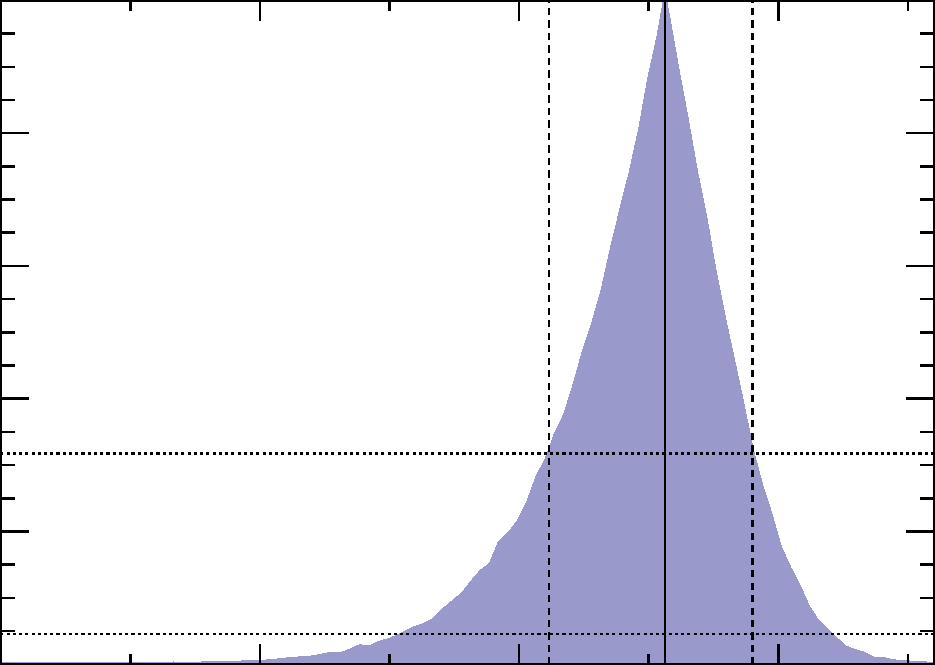
\includegraphics[width=0.9\textwidth]{Vub/Gamma/gammacombo_g}};
        \begin{scope}[x={(image.south east)},y={(image.north west)}]
            \foreach \x in {0, ..., 2}
            {
                \tikzmath{\xtext = (\x + 1) * 50; \xcoord = \x * .276 + .280;}
                \node at (\xcoord, -0.040) {\(\pgfmathprintnumber[fixed,precision=0,fixed zerofill=true]{\xtext}\)};
            }
            \node[anchor=east] at (0.005, 0.0) {\num{0}};
            \foreach \y in {1, ..., 4}
            {
                \tikzmath{\ytext = \y / 5; \ycoord = \y / 5;}
                \node[anchor=east] at (0.005, \ycoord) {\(\pgfmathprintnumber[fixed,precision=1,fixed zerofill=true]{\ytext}\)};
            }
            \node[anchor=east] at (0.005, 1.0) {\num{1}};
            \node[anchor=east] at (1.0, -0.10) {\CPgamma [\SIUnitSymbolDegree]};
            \node[rotate=90,anchor=east,inner xsep=0pt,outer xsep=0pt] at (-0.12, 1.0) {\omcl};
            \node[anchor=base west] at (0.270, 0.585) {\ang[parse-numbers=false]{\left(128_{-22}^{+17}\right)}};
            \node[anchor=base west] at (0.127, 0.338) {\SI{68.3}{\percent}};
            \node[anchor=base west] at (0.127, 0.066) {\SI{95.5}{\percent}};
            \node[anchor=base west] at (0.06, 0.823) {\lhcb};
        \end{scope}
    \end{tikzpicture}
    \caption{
        Confidence levels of the various values of~\CPgamma, with the apex at the maximum likelihood of~\ang{128}.
        The \num{1}~and \num{2}~standard deviations intervals are also indicated.}
    \label{fig:Vub_gamma}
\end{figure}
%
\begin{figure}[hp] \centerfloat
    \hspace*{-.75cm}
    \fontsize{8}{9.6}\selectfont
    \begin{subfigure}{.48\textwidth}
        \begin{tikzpicture}
            \node[anchor=south west,inner sep=0] (image) at (0,0) {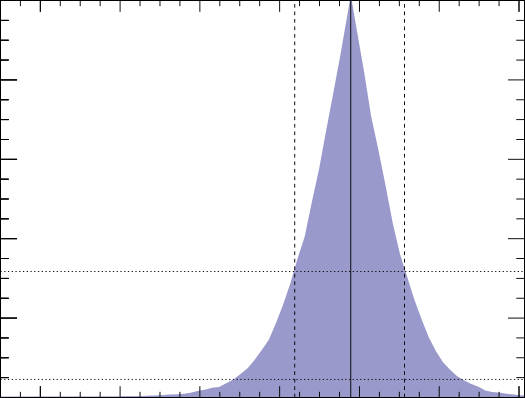
\includegraphics[width=0.9\textwidth]{Vub/Gamma/gammacombo_d_dsk}};
            \begin{scope}[x={(image.south east)},y={(image.north west)}]
                \foreach \x in {0, ..., 6}
                {
                    \tikzmath{\xtext = \x * 20 + 280; \xcoord = \x * .151 + .078;}
                    \node at (\xcoord, -0.040) {\(\pgfmathprintnumber[fixed,precision=0,fixed zerofill=true]{\xtext}\)};
                }
                \node[anchor=east] at (0.005, 0.0) {\num{0}};
                \foreach \y in {1, ..., 4}
                {
                    \tikzmath{\ytext = \y / 5; \ycoord = \y / 5;}
                    \node[anchor=east] at (0.005, \ycoord) {\(\pgfmathprintnumber[fixed,precision=1,fixed zerofill=true]{\ytext}\)};
                }
                \node[anchor=east] at (0.005, 1.0) {\num{1}};
                \node[anchor=east] at (1.0, -0.12) {\strongangle [\SIUnitSymbolDegree]};
                \node[rotate=90,anchor=east,inner xsep=0pt,outer xsep=0pt] at (-0.12, 1.0) {\omcl};
                \node[anchor=base west] at (0.320, 0.585) {\ang[parse-numbers=false]{\left(358_{-14}^{+13}\right)}};
                \node[anchor=base west] at (0.127, 0.338) {\SI{68.3}{\percent}};
                \node[anchor=base west] at (0.127, 0.066) {\SI{95.5}{\percent}};
                \node[anchor=base west] at (0.06, 0.823) {\large\lhcb};
            \end{scope}
        \end{tikzpicture}
    \end{subfigure} \hfill%
    \begin{subfigure}{.48\textwidth}
        \begin{tikzpicture}
            \node[anchor=south west,inner sep=0] (image) at (0,0) {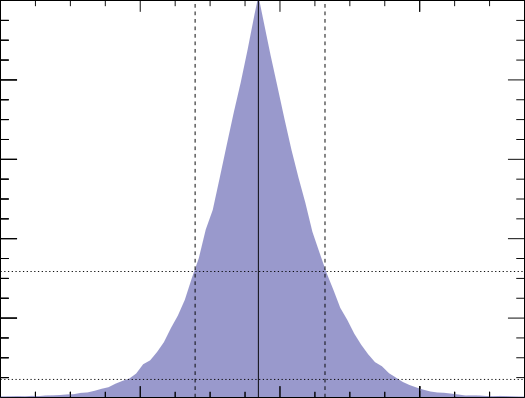
\includegraphics[width=0.9\textwidth]{Vub/Gamma/gammacombo_l_dsk}};
            \begin{scope}[x={(image.south east)},y={(image.north west)}]
                \foreach \x in {0, ..., 3}
                {
                    \tikzmath{\xtext = \x * 0.2; \xcoord = \x * .266;}
                    \node at (\xcoord, -0.040) {\(\pgfmathprintnumber[fixed,precision=1,fixed zerofill=true]{\xtext}\)};
                }
                \node[anchor=east] at (0.005, 0.0) {\num{0}};
                \foreach \y in {1, ..., 4}
                {
                    \tikzmath{\ytext = \y / 5; \ycoord = \y / 5;}
                    \node[anchor=east] at (0.005, \ycoord) {\(\pgfmathprintnumber[fixed,precision=1,fixed zerofill=true]{\ytext}\)};
                }
                \node[anchor=east] at (0.005, 1.0) {\num{1}};
                \node[anchor=east] at (1.0, -0.12) {\rdsk};
                \node[rotate=90,anchor=east,inner xsep=0pt,outer xsep=0pt] at (-0.12, 1.0) {\omcl};
                \node[anchor=base west] at (0.645, 0.585) {\(0.369_{-0.090}^{+0.095}\)};
                \node[anchor=base west] at (0.127, 0.338) {\SI{68.3}{\percent}};
                \node[anchor=base west] at (0.127, 0.066) {\SI{95.5}{\percent}};
                \node[anchor=base west] at (0.06, 0.823) {\large\lhcb};
            \end{scope}
        \end{tikzpicture}
    \end{subfigure}
    \caption{
        Confidence levels of the various values of~\strongangle and~\rdsk.
        The \num{1}~and \num{2}~standard deviations intervals are also indicated.}
    \label{fig:Vub_delta_rdsk}
\end{figure}
%
\begin{figure}[hp] \centerfloat
    \fontsize{18}{21.6}\selectfont
    \begin{tikzpicture}
        \node[anchor=south west,inner sep=0] (image) at (0,0) {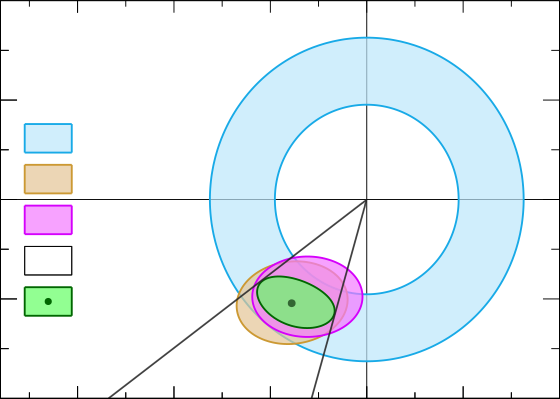
\includegraphics[width=0.9\textwidth]{Vub/Gamma/Lambda_f}};
        \begin{scope}[x={(image.south east)},y={(image.north west)}]
            \node at (0.139 + 0 * 0.172 - 0.02, -0.040) {\num{-1.5}};
            \node at (0.139 + 1 * 0.172 - 0.02, -0.040) {\num{-1}};
            \node at (0.139 + 2 * 0.172 - 0.02, -0.040) {\num{-0.5}};
            \node at (0.139 + 3 * 0.172, -0.040) {\num{0}};
            \node at (0.139 + 4 * 0.172, -0.040) {\num{0.5}};
            \node at (1.0, -0.040) {\num{1}};
            \node[anchor=east] at (0.005, 0.00) {\num{-1}};
            \node[anchor=east] at (0.005, 0.25) {\num{-0.5}};
            \node[anchor=east] at (0.005, 0.50) {\num{ 0}};
            \node[anchor=east] at (0.005, 0.75) {\num{ 0.5}};
            \node[anchor=east] at (0.005, 1.00) {\num{ 1}};

            % Legend
            {
                \fontsize{12}{14.4}\selectfont
                \node[anchor=base west] at (0.130, 0.640) {\(\sqrt{1 - \Cpar^{2}}\)};
                \node[anchor=base west] at (0.130, 0.640 - 1 * 0.103) {\({(-\Dpar, \Spar)}\)};
                \node[anchor=base west] at (0.130, 0.640 - 2 * 0.103) {\({(-\Dbpar, \Sbpar)}\)};
                \node[anchor=base west] at (0.130, 0.640 - 3 * 0.103) {\({-\left(\weak\right)}\)};
                \node[anchor=base west] at (0.130, 0.640 - 4 * 0.103) {Combination};
            }

            \node[anchor=east] at (1.0, -0.155) {\({\Im\left[2\lf / (1 + \abs{\lf}^{2})\right]}\)};
            \node[rotate=90,anchor=east,inner xsep=0pt,outer xsep=0pt] at (-0.14, 1.0) {\({\Re\left[2\lf / (1 + \abs{\lf}^{2})\right]}\)};
            \node[anchor=base west] at (0.06, 0.823) {\lhcb};
        \end{scope}
    \end{tikzpicture}
    \caption{
        Real and imaginary parts of the parameter~\lf, given in \cref{eqn:Vub_lambdaf}.
        The constraints given by the \CP-violation parameters are indicated, as well as the combined result.}
    \label{fig:Vub_lambdaf}
\end{figure}

\clearpage
\subsection{Outlook}
\label{sec:Vub_Outlook}

The uncertainty on the value of~\CPgamma obtained in the previous \lcnamecref{sec:Vub_gamma} is limited by the amount of data available.
Therefore, it is interesting to study how this uncertainty will evolve as more data from the \lhcb~detector becomes available.

The current total uncertainty on~\CPgamma with this method is about~\ang{20}, including both statistical and systematic sources of uncertainty.
These can not be trivially separated, but from the separate uncertainties on the \CP-violation observables (see \cref{eqn:BsDsK_TD_Results}), it can be estimated that the statistical component dominates.
It is taken as the sole contribution of uncertainties in the following argument.

By the end of the second \lhc~run, in 2018, the total data is expected to have increased from~\SI{3}{\per\femto\barn} to~\SI{9}{\per\femto\barn}.
This yields an expected statistical uncertainty of~\ang{12} at that point in time, comparable to the current systematic uncertainty of~\ang{12}.
The challenge for the analysis using this data is thus to control the sources of systematic uncertainty.
The main contributions of systematic uncertainties arise from correlations between the decay-time and variables entering the multivariate fit, as well as the combination of decay-time resolution and flavour tagging.
The former could be controlled with a different method of selecting signal candidates, for example through the use of machine learning.
The latter will decrease as larger resolution calibration samples and more sophisticated flavour tagging algorithms become are developed.

In a realistically possible scenario, when the systematic uncertainty decreases to \eg~\ang{8}, this could lead to a total uncertainty of about~\ang{14}.
In that case, the channel~\BsDsK presents a significant contribution to the \CPgamma~combination, which is expected to decrease to about~\ang{4} by that time~\cite{LHCb-PAPER-2016-032}, driven by decays of \Bpm~mesons of the form \decay{\Bpm}{\Dz\Kpm}.
This accuracy is also sufficient to solve the current discrepancy between the values of~\CPgamma from \BsDsK~decays and other \bquark~meson decays.

Using even more data from the \lhcb~upgrade era and a significant reduction of the systematic uncertainty from a better understanding of the detector, a precision of about~\ang{1} is expected to be attained.
An effect that can start to play a role at that time is the pollution of penguin topologies in the calculation of~\betas, neglected in the assumption~\({\phis = -2\betas}\).
Within current experimental and theoretical limits, this effect can be of a magnitude up to~\({\abs{\upDelta\phis} = \ang{1}}\)~\cite{VSyropoulos:PhDThesis,DeBruyn:PhDThesis,DeBruyn:2014oga}.
Therefore, it is important to understand the contribution of penguin topologies.

\clearpage
\section{\abs{\Vub}~from \BdDsPi~and \LbDsP}
\label{sec:VubDsH}

Until now, the discussion in this thesis has focused on the phase of the CKM~element~\Vub.
In this \lcnamecref{sec:VubDsH}, measurements regarding the magnitude of~\Vub are discussed.

At tree level, the decay channels~\BdDsPi and~\LbDsP are dominated by a \bquark~hadron decaying to a light hadron (\pip~or \proton) while emitting a \Dsm~through the weak interaction, as depicted in \cref{fig:Vub_FeynmanDiagrams}.
These decays proceed through the CKM~element~\Vub, and are therefore suppressed compared to similar decays, such as~\BsDsPi.

The branching fractions of these decays are proportional to~\(\abs{\Vub}^{2} \abs{\aNF}^{2}\) (see \cref{sec:theory_WeakDecays}), and as such measuring them can yield information on both~\(\abs{\Vub}\) and the nonfactorisation factor~\(\abs{\aNF}\).
The current \lcnamecref{sec:VubDsH} describes such measurements, each done using data collected by the \lhcb~detector corresponding to an integrated luminosity of \SI{5}{\per\femto\barn}.
This includes the same~\SI{3}{\per\femto\barn} described in \cref{chp:DsK_BF,chp:BsDsK_TD}, and and additional~\SI{2}{\per\femto\barn} taken at \({\sqs = \SI{13}{\TeV}}\).
%
\begin{table}[htb] \centerfloat
    \caption{
        Total selection efficiencies for both signal channels and both control channels, split by centre-of-mass energy.}
    \label{tab:Vub_Efficiencies}
    \rowcolors{1}{tableshade}{}
    \begin{tabular}{l*{2}{S[table-format=1.4(4)]}}
        \hiderowcolors \toprule
        \multirow{2}{*}[-2pt]{Decay~channel} & \multicolumn{2}{c}{Total selection efficiency~(\si{\percent})} \tabularnewline
        \cmidrule(lr){2-3}
                & {\(\sqs = \SI[parse-numbers=false]{7, 8}{\TeV}\)} & {\(\sqs = \SI{13}{\TeV}\)} \tabularnewline
        \showrowcolors \midrule
        \BdDsPi & 0.1543 +- 0.0010 & 0.2014 +- 0.0012 \tabularnewline
        \BdDPi  & 0.3569 +- 0.0020 & 0.4368 +- 0.0010 \tabularnewline
        \midrule
        \LbDsP  & 0.1045 +- 0.0006 & 0.2215 +- 0.0009 \tabularnewline
        \LbLcPi & 0.1135 +- 0.0002 & 0.3755 +- 0.0007 \tabularnewline
        \bottomrule
    \end{tabular}
\end{table}
%
\begin{figure}[htb] \centerfloat
    \begin{subfigure}{\textwidth} \centerfloat
        \begin{tikzpicture}
            \setlength{\diagramsize}{3.5em}
            \setlength{\diagramheight}{\baselineskip}
            \begin{feynman}
                \vertex (a1);
                \vertex[right=2\diagramsize of a1] (a2);
                \vertex[right=2\diagramsize of a2] (a3) {\dquark};

                \vertex[below=\diagramheight of a1] (b1);
                \vertex[right=2\diagramsize of b1] (b2);
                \vertex[right=2\diagramsize of b2] (b3) {\dquark};

                \vertex[above right=4\diagramheight and \diagramsize of a2] (x1);
                \vertex[above right=1.25\diagramheight and \diagramsize of x1] (x2);
                \vertex[below right=1.25\diagramheight and \diagramsize of x1] (x3);

                \diagram* {
                    {[edges=fermion]
                    (a3) -- (a2) -- (a1),
                    (b1) -- (b3),
                    (x1) -- (x2),
                    (x3) -- (x1),
                    },
                    (a2) -- [boson, edge label={\Wp}] (x1),
                };

                \node[at=(b1), anchor=mid east] (q1) {\dquark};
                \node[at=(q1.mid |- a1), anchor=mid] (b) {\bquark};

                \node[at=(x2), anchor=mid west] (m1) {\cquark};
                \node[at=(x3), anchor=mid west] (m2) {\squark};

                \draw [decoration={brace}, decorate] (q1.south west) -- (q1.south west |- b.north west) node [midway, left, outer xsep=.05\diagramsize] {\Bd};
                \draw [decoration={brace}, decorate] (a3.north east -| b3.south east) -- (b3.south east) node [midway, right, outer xsep=.05\diagramsize] {\pim};
                \draw [decoration={brace}, decorate] (b3.south east |- m1.north east) -- (b3.south east |- m2.south east) node [midway, right, outer xsep=.05\diagramsize] {\Dsp};
            \end{feynman}
        \end{tikzpicture}
        \caption{Diagram of the decay~\BdDsPi.}
    \end{subfigure}
    \\[4ex]
    \begin{subfigure}{\textwidth} \centerfloat
        \begin{tikzpicture}
            \setlength{\diagramsize}{3.5em}
            \setlength{\diagramheight}{\baselineskip}
            \begin{feynman}
                \vertex (a1);
                \vertex[right=2\diagramsize of a1] (a2);
                \vertex[right=2\diagramsize of a2] (a3) {\uquark};

                \vertex[below=\diagramheight of a1] (b1);
                \vertex[right=2\diagramsize of b1] (b2);
                \vertex[right=2\diagramsize of b2] (b3) {\uquark};

                \vertex[below=\diagramheight of b1] (c1);
                \vertex[right=2\diagramsize of c1] (c2);
                \vertex[right=2\diagramsize of c2] (c3) {\dquark};

                \vertex[above right=4\diagramheight and \diagramsize of a2] (x1);
                \vertex[above right=1.25\diagramheight and \diagramsize of x1] (x2);
                \vertex[below right=1.25\diagramheight and \diagramsize of x1] (x3);

                \diagram* {
                    {[edges=fermion]
                    (a1) -- (a2) -- (a3),
                    (b1) -- (b3),
                    (c1) -- (c3),
                    (x1) -- (x2),
                    (x3) -- (x1),
                    },
                    (a2) -- [boson, edge label=\(\Wm\)] (x1),
                };

                \node[at=(c1), anchor=mid east] (q2) {\dquark};
                \node[at=(q2.mid |- b1), anchor=mid] (q1) {\uquark};
                \node[at=(q1.mid |- a1), anchor=mid] (b) {\bquark};

                \node[at=(x2), anchor=mid west] (m1) {\squark};
                \node[at=(x3), anchor=mid west] (m2) {\dquark};

                \draw [decoration={brace}, decorate] (q2.south west) -- (q2.south west |- b.north west) node [midway, left, outer xsep=.05\diagramsize] {\Lb};
                \draw [decoration={brace}, decorate] (a3.north east -| c3.south east) -- (c3.south east) node [midway, right, outer xsep=.05\diagramsize] {\proton};
                \draw [decoration={brace}, decorate] (c3.south east |- m1.north east) -- (c3.south east |- m2.south east) node [midway, right, outer xsep=.05\diagramsize] {\Dsm};
            \end{feynman}
        \end{tikzpicture}
        \caption{Diagram of the decay~\LbDsP.}
    \end{subfigure}
    \caption{
        Diagrams of the decays~\BdDsPi and~\LbDsP.}
    \label{fig:Vub_FeynmanDiagrams}
\end{figure}
%
\begin{figure}[p] \centerfloat
    \fontsize{6}{7.2}\selectfont
    \begin{subfigure}{.48\textwidth} \centerfloat
        \begin{tikzpicture}
            \node[anchor=south west,inner sep=0] (image) at (0,0) {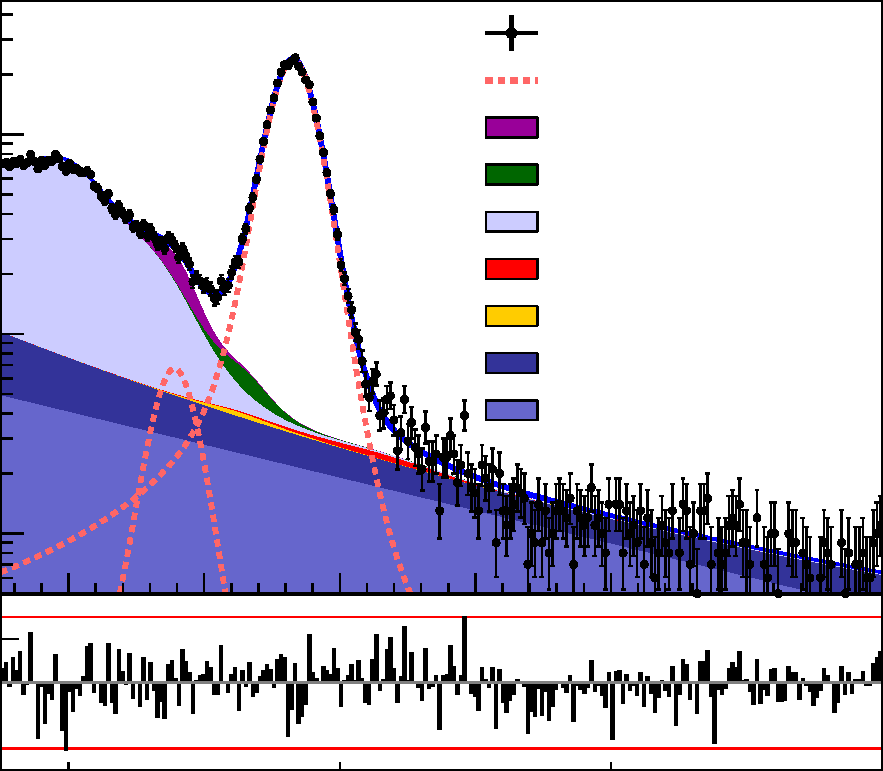
\includegraphics[width=0.85\textwidth]{Vub/BFs/mass_Bs2DsPi_BeautyMass_both_phipi_run1_log_IpJo_final3}};
            \begin{scope}[x={(image.south east)},y={(image.north west)}]
                \foreach \x in {0, ..., 3}
                {
                    \tikzmath{\xpos = (\x / 3) * (1. - 0.079) + 0.079; \xtext = 5200 + 200 * \x;}
                    \node at (\xpos, -0.025) {\pgfmathprintnumber[fixed,precision=0,fixed zerofill=true,1000 sep={}]{\xtext}};
                }
                \node[anchor=base east] at (0.005, 0.297       ) {\num{10}};
                \node[anchor=base east] at (0.005, 0.297+1*.257) {\num{e2}};
                \node[anchor=base east] at (0.005, 0.297+2*.257) {\num{e3}};
                \foreach \p in {1, ..., 3}
                {
                    \tikzmath{\ypos = (\p / 4) * 0.230; \ptext = (\p - 2) * 2;}
                    \node[anchor=east] at (0.005, \ypos) {\(\scriptstyle\pgfmathprintnumber[fixed,precision=0,fixed zerofill=true]{\ptext}\)};
                }
                {
                    \fontsize{8}{9.6}\selectfont
                    \node[anchor=east] at (1.0, -0.11) {\({m(\DsmpPipm)}~[\si{\MeVcc}]\)};
                    \node[rotate=90,anchor=east,inner xsep=0pt,outer xsep=0pt] at (-0.11, 1.0) {\({\text{Candidates}/(\SI{2.6}{\MeVcc})}\)};
                }
                \node[anchor=west] at (0.06, 0.92) {\large\lhcb};
                % Legend
                {
                    \fontsize{5}{6}\selectfont
                    \node[anchor=base west] at (0.605, 0.943) {Data};
                    \node[anchor=base west] at (0.605, 0.943 - 1 * 0.0607) {\BdorBsDsPi~signal};
                    \node[anchor=base west] at (0.605, 0.943 - 2 * 0.0607) {\BdDsPi~signal};
                    \node[anchor=base west] at (0.605, 0.943 - 3 * 0.0607) {\BsDsK};
                    \node[anchor=base west] at (0.605, 0.943 - 4 * 0.0607) {\decay{\Bs}{\DsorDssm(\pip, \rhop)}};
                    \node[anchor=base west] at (0.605, 0.943 - 5 * 0.0607) {\LbLcPi};
                    \node[anchor=base west] at (0.605, 0.943 - 6 * 0.0607) {\BdDPi};
                    \node[anchor=base west] at (0.605, 0.943 - 7 * 0.0607) {Comb.~random~\Dsm};
                    \node[anchor=base west] at (0.605, 0.943 - 8 * 0.0607) {Comb.~true~\Dsm};
                }
            \end{scope}
        \end{tikzpicture}
        \caption{Fit to the \DspmPimp~invariant mass, \({\sqs = \SI[parse-numbers=false]{7, 8}{\TeV}}\).}
    \end{subfigure} \hfill%
    \begin{subfigure}{.48\textwidth} \centerfloat
        \begin{tikzpicture}
            \node[anchor=south west,inner sep=0] (image) at (0,0) {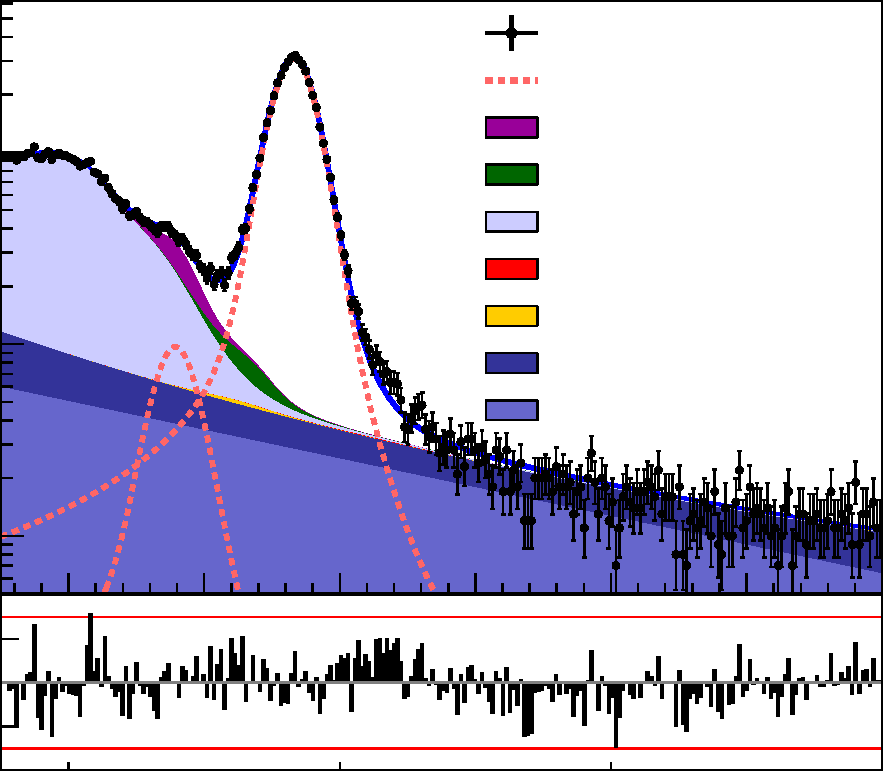
\includegraphics[width=0.85\textwidth]{Vub/BFs/mass_Bs2DsPi_BeautyMass_both_phipi_run2_log_IpJo_final3}};
            \begin{scope}[x={(image.south east)},y={(image.north west)}]
                \foreach \x in {0, ..., 3}
                {
                    \tikzmath{\xpos = (\x / 3) * (1. - 0.079) + 0.079; \xtext = 5200 + 200 * \x;}
                    \node at (\xpos, -0.025) {\pgfmathprintnumber[fixed,precision=0,fixed zerofill=true,1000 sep={}]{\xtext}};
                }
                \node[anchor=base east] at (0.005, 0.291       ) {\num{10}};
                \node[anchor=base east] at (0.005, 0.291+1*.247) {\num{e2}};
                \node[anchor=base east] at (0.005, 0.291+2*.247) {\num{e3}};
                \foreach \p in {1, ..., 3}
                {
                    \tikzmath{\ypos = (\p / 4) * 0.230; \ptext = (\p - 2) * 2;}
                    \node[anchor=east] at (0.005, \ypos) {\(\scriptstyle\pgfmathprintnumber[fixed,precision=0,fixed zerofill=true]{\ptext}\)};
                }
                {
                    \fontsize{8}{9.6}\selectfont
                    \node[anchor=east] at (1.0, -0.11) {\({m(\DsmpPipm)}~[\si{\MeVcc}]\)};
                    \node[rotate=90,anchor=east,inner xsep=0pt,outer xsep=0pt] at (-0.11, 1.0) {\({\text{Candidates}/(\SI{2.6}{\MeVcc})}\)};
                }
                \node[anchor=west] at (0.06, 0.92) {\large\lhcb};
                % Legend
                {
                    \fontsize{5}{6}\selectfont
                    \node[anchor=base west] at (0.605, 0.943) {Data};
                    \node[anchor=base west] at (0.605, 0.943 - 1 * 0.0607) {\BdorBsDsPi~signal};
                    \node[anchor=base west] at (0.605, 0.943 - 2 * 0.0607) {\BdDsPi~signal};
                    \node[anchor=base west] at (0.605, 0.943 - 3 * 0.0607) {\BsDsK};
                    \node[anchor=base west] at (0.605, 0.943 - 4 * 0.0607) {\decay{\Bs}{\DsorDssm(\pip, \rhop)}};
                    \node[anchor=base west] at (0.605, 0.943 - 5 * 0.0607) {\LbLcPi};
                    \node[anchor=base west] at (0.605, 0.943 - 6 * 0.0607) {\BdDPi};
                    \node[anchor=base west] at (0.605, 0.943 - 7 * 0.0607) {Comb.~random~\Dsm};
                    \node[anchor=base west] at (0.605, 0.943 - 8 * 0.0607) {Comb.~true~\Dsm};
                }
            \end{scope}
        \end{tikzpicture}
        \caption{Fit to the \DspmPimp~invariant mass, \({\sqs = \SI{13}{\TeV}}\).}
    \end{subfigure}
    \\[4ex]
    \begin{subfigure}{.48\textwidth} \centerfloat
        \begin{tikzpicture}
            \node[anchor=south west,inner sep=0] (image) at (0,0) {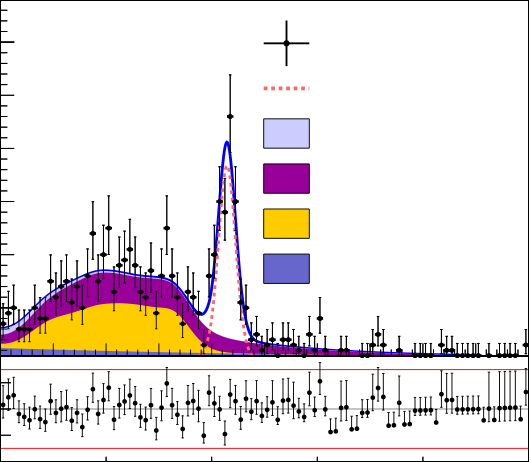
\includegraphics[width=0.85\textwidth]{Vub/BFs/mass_Lb2Dsp_BeautyMass_kkpi_both_run1}};
            \begin{scope}[x={(image.south east)},y={(image.north west)}]
                \foreach \x in {0, ..., 5}
                {
                    \tikzmath{\xpos = (\x / 5); \xtext = 5200 + 200 * \x;}
                    \node at (\xpos, -0.025) {\pgfmathprintnumber[fixed,precision=0,fixed zerofill=true,1000 sep={}]{\xtext}};
                }
                \foreach \y in {0, ..., 5}
                {
                    \tikzmath{\ypos = (\y / 5) * 0.573 + 0.318; \ytext = 10 * \y + 10;}
                    \node[anchor=base east] at (0.005, \ypos) {\(\pgfmathprintnumber[fixed,precision=0,fixed zerofill=true]{\ytext}\)};
                }
                \foreach \p in {1, ..., 3}
                {
                    \tikzmath{\ypos = (\p / 4) * 0.230; \ptext = (\p - 2) * 2;}
                    \node[anchor=east] at (0.005, \ypos) {\(\scriptstyle\pgfmathprintnumber[fixed,precision=0,fixed zerofill=true]{\ptext}\)};
                }
                {
                    \fontsize{8}{9.6}\selectfont
                    \node[anchor=east] at (1.0, -0.11) {\({m(\DsmpPpm)}~[\si{\MeVcc}]\)};
                    \node[rotate=90,anchor=east,inner xsep=0pt,outer xsep=0pt] at (-0.11, 1.0) {\({\text{Candidates}/(\SI{10}{\MeVcc})}\)};
                }
                \node[anchor=west] at (0.06, 0.92) {\large\lhcb};
                % Legend
                {
                    \fontsize{5}{6}\selectfont
                    \node[anchor=base west] at (0.591, 0.893) {Data};
                    \node[anchor=base west] at (0.591, 0.893 - 1 * 0.0977) {\LbDsP~signal};
                    \node[anchor=base west] at (0.591, 0.893 - 2 * 0.0977) {\BsDsOrDsstKorKst};
                    \node[anchor=base west] at (0.591, 0.893 - 3 * 0.0977) {\decay{\Bs}{\DsorDssm(\pip, \rhop)}};
                    \node[anchor=base west] at (0.591, 0.893 - 4 * 0.0977) {\LbDsstP};
                    \node[anchor=base west] at (0.591, 0.893 - 5 * 0.0977) {Combinatorial};
                }
            \end{scope}
        \end{tikzpicture}
        \caption{Fit to the \DsmpPpm~invariant mass, \({\sqs = \SI[parse-numbers=false]{7, 8}{\TeV}}\).}
    \end{subfigure} \hfill%
    \begin{subfigure}{.48\textwidth} \centerfloat
        \begin{tikzpicture}
            \node[anchor=south west,inner sep=0] (image) at (0,0) {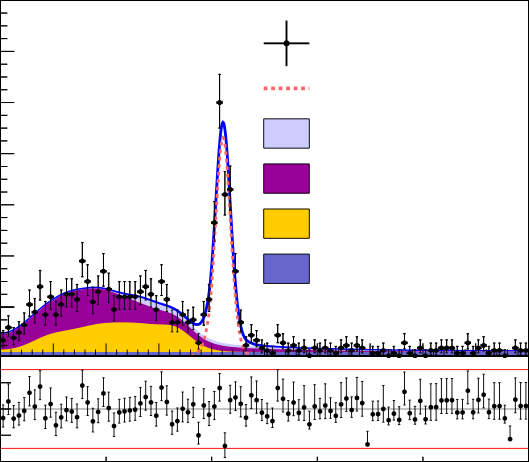
\includegraphics[width=0.85\textwidth]{Vub/BFs/mass_Lb2Dsp_BeautyMass_kkpi_both_run2}};
            \begin{scope}[x={(image.south east)},y={(image.north west)}]
                \foreach \x in {0, ..., 5}
                {
                    \tikzmath{\xpos = (\x / 5); \xtext = 5200 + 200 * \x;}
                    \node at (\xpos, -0.025) {\pgfmathprintnumber[fixed,precision=0,fixed zerofill=true,1000 sep={}]{\xtext}};
                }
                \foreach \y in {0, ..., 5}
                {
                    \tikzmath{\ypos = (\y / 5) * 0.551 + 0.321; \ytext = 10 * \y + 10;}
                    \node[anchor=base east] at (0.005, \ypos) {\(\pgfmathprintnumber[fixed,precision=0,fixed zerofill=true]{\ytext}\)};
                }
                \foreach \p in {1, ..., 3}
                {
                    \tikzmath{\ypos = (\p / 4) * 0.230; \ptext = (\p - 2) * 2;}
                    \node[anchor=east] at (0.005, \ypos) {\(\scriptstyle\pgfmathprintnumber[fixed,precision=0,fixed zerofill=true]{\ptext}\)};
                }
                {
                    \fontsize{8}{9.6}\selectfont
                    \node[anchor=east] at (1.0, -0.11) {\({m(\DsmpPpm)}~[\si{\MeVcc}]\)};
                    \node[rotate=90,anchor=east,inner xsep=0pt,outer xsep=0pt] at (-0.11, 1.0) {\({\text{Candidates}/(\SI{10}{\MeVcc})}\)};
                }
                \node[anchor=west] at (0.06, 0.92) {\large\lhcb};
                % Legend
                {
                    \fontsize{5}{6}\selectfont
                    \node[anchor=base west] at (0.591, 0.893) {Data};
                    \node[anchor=base west] at (0.591, 0.893 - 1 * 0.0977) {\LbDsP~signal};
                    \node[anchor=base west] at (0.591, 0.893 - 2 * 0.0977) {\BsDsOrDsstKorKst};
                    \node[anchor=base west] at (0.591, 0.893 - 3 * 0.0977) {\decay{\Bs}{\DsorDssm(\pip, \rhop)}};
                    \node[anchor=base west] at (0.591, 0.893 - 4 * 0.0977) {\LbDsstP};
                    \node[anchor=base west] at (0.591, 0.893 - 5 * 0.0977) {Combinatorial};
                }
            \end{scope}
        \end{tikzpicture}
        \caption{Fit to the \DsmpPpm~invariant mass, \({\sqs = \SI{13}{\TeV}}\).}
    \end{subfigure}
    \caption{
        Mass fits to determine the yields of the decays~\BdDsPi and~\LbDsP.
        Note that in the fits to the \DspmPimp~invariant mass, the decay under study,~\BdDsPi, appears as the small purple-shaded peak on the left-hand side of the dominating \BsDsPi~mass peak.}
    \label{fig:Vub_MassFits}
\end{figure}

The decay channel~\BdDsPi is reconstructed using~\DsmKKPi and normalised to~\BdDPi (with~\DmKPiPi), while \LbDsP (with~\DsmKKPi) is normalised to \LbLcPi (with~\LcPKPi).
These normalisation channels are Cabibbo-allowed, and are chosen to allow a determination of the branching fractions without having to take into account differences in \bquark-hadron production.
The yields and efficiencies are mostly determined analogous to the procedures described in \cref{chp:DsK_BF}~\cite{JButter:MasterThesis,MTervoert:MasterThesis}.
The mass fits are shown in \cref{fig:Vub_MassFits}, their accompanying yields in \cref{tab:Vub_Yields}, and the efficiencies in \cref{tab:Vub_Efficiencies}.
Together, they result in the following branching fractions:
%
\begin{align}
    \BF(\BdDsPi) &=   \num{23.1 +- 2.3 e-6} \rlap{,} \\
    \BF(\LbDsP)  &= \0\num{ 7.5 +- 0.8 e-6} \rlap{,}
\end{align}
%
where the errors are a combination of statistical errors and errors on external inputs.
This is a first observation of the decay~\LbDsP, and the branching fraction of~\BdDsPi is of the same precision as the current world-average value~\cite{PDG}.
%
\begin{table}[htb] \centerfloat
    \caption{
        Signal yields from the mass fits shown in \cref{fig:Vub_MassFits}.}
    \label{tab:Vub_Yields}
    \rowcolors{1}{tableshade}{}
    \begin{tabular}{lS[table-format=6(4)]S[table-format=6(4)]S[table-format=7(4)]}
        \hiderowcolors \toprule
        \multirow{2}{*}[-2pt]{Decay~channel} & \multicolumn{3}{c}{Yield} \tabularnewline
        \cmidrule(lr){2-4}
                & {\(\sqs = \SI[parse-numbers=false]{7, 8}{\TeV}\)} & {\(\sqs = \SI{13}{\TeV}\)} & {Total} \tabularnewline
        \showrowcolors \midrule
        \BdDsPi &   1035 +-  118 &   1648 +-  157 &    2683 +- 196 \tabularnewline
        \BdDPi  & 500842 +- 1167 & 584929 +- 1619 & 1085771 +- 1996 \tabularnewline
        \midrule
        \LbDsP  &    158 +-   11 &    334 +-   18 &     492 +- 21 \tabularnewline
        \LbLcPi &  98591 +-  344 & 219033 +-  587 &  317624 +- 680 \tabularnewline
        \bottomrule
    \end{tabular}
\end{table}

The branching fraction of~\BdDsPi can be related to~\({\absx{\Vub} \absx{\aNF^{\BdDsPi}}}\) using \cref{eqn:theory_BF}, by using external input for the form factor~\cite{Ball:2004ye,Ball:2006jz},
%
\begin{equation}
    {F_{\decay{\Bd}{\pim}} |_{q^{2}=m_{\Dspm}^{2}} = \num{0.333 +- 0.026}} \rlap{,}
\end{equation}
%
as well as for the decay constant~\cite{Bazavov:2017lyh},
%
\begin{equation}
    {f_{\Dspm} = \SI{0.2498 +- 0.0003}{\GeV}} \rlap{,}
\end{equation}
%
resulting in
%
\begin{equation}
    {\absx{\Vub} \absx{\aNF^{\BdDsPi}} = \num{3.34 +- 0.32 e-3}} \rlap{.}
\end{equation}
%
This value allows extraction of~\(\absx{\aNF^{\BdDsPi}}\) by using the current world-average value of~\(\absx{\Vub}\)~\cite{PDG}, \({\absx{\Vub} = \num{3.94 +- 0.36 e-3}}\),
%
\begin{equation}
    \absx{\aNF^{\BdDsPi}} = \num{0.86 +- 0.11} \rlap{.}
\end{equation}
%
This result is compatible with naive factorisation, but also allows for a sizeable nonfactorisable effect.

In principle, the inverse is also possible: fixing~\(\absx{\aNF}\) in order to determine~\(\absx{\Vub}\).
However, current knowledge of~\(\aNF\) in the case of a light decay product in the form factor and a heavy one in the decay constant, as is the case here, is limited.
It is possible to assume naive factorisation,~\(\absx{\aNF^{\BdDsPi}}\), using an associated error of~\SI{20}{\percent}, resulting in
%
\begin{equation}
    \absx{\Vub} = \num{3.34 +- 0.74 e-3} \rlap{,}
\end{equation}
%
which is compatible with both the current exclusive and inclusive values for~\(\absx{\Vub}\), though the central value is closer to that of the exclusive determination.
While the uncertainties are too large for now, this may provide another handle for differentiating between the inclusive and exclusive~\(\absx{\Vub}\) values, especially if~\(\aNF\) can be externally constrained.

Both approaches, with external input for~\(\absx{\Vub}\) split between inclusive, exclusive, and average measurements, are shown in \cref{fig:Vub_aNFVub}.
%
\begin{figure}[htb] \centerfloat
    \begin{tikzpicture}
        \node[anchor=south west,inner sep=0] (image) at (0,0) {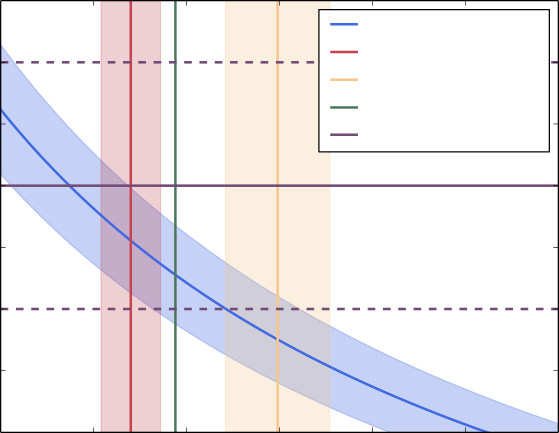
\includegraphics[width=0.86\textwidth]{Vub/BFs/Plot_result}};
        \begin{scope}[x={(image.south east)},y={(image.north west)}]
            \foreach \x in {0, ..., 6}
            {
                \tikzmath{\xpos = \x / 6.; \xtext = \x * 0.0005 + 0.0030;}
                \node at (\xpos, -0.027) {\(\pgfmathprintnumber[fixed,precision=4,fixed zerofill=true]{\xtext}\)};
            }
            \node[anchor=east] at (0.005, 0.008) {\(\pgfmathprintnumber[fixed,precision=1,fixed zerofill=true]{0.6}\)};
            \foreach \y in {1, ..., 7}
            {
                \tikzmath{\ypos = \y / 7.; \ytext = \y * 0.1 + 0.6;}
                \node[anchor=east] at (0.005, \ypos) {\(\pgfmathprintnumber[fixed,precision=1,fixed zerofill=true]{\ytext}\)};
            }
            % Legend
            {
                \node[anchor=base west] at (0.650, 0.935) {\({\abs{\aNF}\abs{\Vub}}\)~result};
                \node[anchor=base west] at (0.650, 0.935 - 1 * 0.065) {\abs{\Vub}~exclusive};
                \node[anchor=base west] at (0.650, 0.935 - 2 * 0.065) {\abs{\Vub}~inclusive};
                \node[anchor=base west] at (0.650, 0.935 - 3 * 0.065) {\abs{\Vub}~average};
                \node[anchor=base west] at (0.650, 0.935 - 4 * 0.065) {Naive factorisation};
            }
            \node[anchor=east] at (1.0, -0.10) {\abs{\Vub}};
            \node[rotate=90,anchor=east,inner xsep=0pt,outer xsep=0pt] at (-0.09, 1.0) {\abs{\aNF}};
        \end{scope}
    \end{tikzpicture}
    \caption{
        Allowed range of~\(\absx{\Vub} \absx{\aNF^{\BdDsPi}}\).
        The vertical lines represent the inclusive, exclusive, and average external measurements of~\(\absx{\Vub}\), and the horizontal lines indicate naive factorisation,~\({\absx{\aNF^{\BdDsPi}} = \num{1 +- .2}}\).
        The curved band is the current measurement of~\({\absx{\Vub} \absx{\aNF^{\BdDsPi}}}\).}
    \label{fig:Vub_aNFVub}
\end{figure}
